\documentclass[10pt,letterpaper]{article}
\usepackage[margin=0.6in]{geometry}
\usepackage[T1]{fontenc}
\usepackage{lmodern}
\usepackage{microtype}
\usepackage{graphicx}
\usepackage{booktabs}
\usepackage{tabularx}
\usepackage{array}
\usepackage{enumitem}
\usepackage{titlesec}
\usepackage{xurl}
\usepackage[hidelinks]{hyperref}
\usepackage{xcolor}

\setlist{nosep,leftmargin=1.1em}
\titleformat{\section}{\normalsize\bfseries}{\thesection.}{0.4em}{}
\titlespacing*{\section}{0pt}{5pt}{1pt}
\setlength{\parindent}{0pt}
\setlength{\parskip}{2pt}
\newcolumntype{L}{>{\raggedright\arraybackslash}X}
\newcolumntype{P}[1]{>{\raggedright\arraybackslash}p{#1}}
\renewcommand{\arraystretch}{1.05}
\newcommand{\todo}[1]{\colorbox{yellow}{\textbf{#1}}}

\begin{document}

\begin{center}
{\large\bfseries StudyLens: Graph-Grounded Diagram Q\&A}\\[2pt]
CECS 458/558 Term Project \textperiodcentered{} Phase 2: Prototype Progress Report\\[1pt]
\textbf{Krish Patel} \textperiodcentered{} November 2026 \textperiodcentered{}
Repository: \url{https://github.com/krish-patel1003/CECS558-term-project-studylens}
\end{center}

\section{Objective and Current Scope}
StudyLens helps students check AI answers about diagrams. It extracts a diagram's entities and arrows into a graph, answers structural questions from that graph, cites the supporting arrow, and abstains when no arrow supports an answer. \textbf{Phase 2 scope:} the MVP loop (upload $\rightarrow$ extract $\rightarrow$ review/correct graph $\rightarrow$ ask $\rightarrow$ grounded answer with highlighted evidence or abstention) and a pilot E2-vs-E3 evaluation on synthetic diagrams. Stretch features from Phase 1 (quizzes, PDFs, history, LoRA) are out of scope.

\section{Completed Features (verified in the repository)}
\begin{itemize}
\item \textbf{Web app} (FastAPI + single-page HTML/JS): PNG/JPEG upload (validated, $\le$5\,MB, processed in memory, never stored); diagram with an SVG overlay of extracted boxes and arrows; editable arrow list; Q\&A panel showing evidence arrows in red, or an ``Abstained'' card.
\item \textbf{AI extraction:} Qwen2.5-VL-3B-Instruct (zero-shot, local, bf16 on Apple M4/MPS) returns JSON entities, boxes and arrows. Our parser repairs the JSON, rescales boxes and drops arrows to unknown entities.
\item \textbf{Graph QA (not AI):} rule-based question typing + NetworkX for direct inputs/outputs, upstream/downstream, arrow check (reports reversed arrows), path, counts and start/end. It abstains on unknown entities, non-structural questions or empty results.
\item \textbf{Clearly labelled non-AI fallback} (\texttt{EXTRACTOR\_BACKEND=annotation}) returns gold graphs for bundled samples, so graders can run the UI without the 7.5\,GB model.
\item \textbf{Baseline E2} in the UI (``ask the VLM directly'') and an \textbf{evaluation harness} (E2/E3/E3*, extraction P/R/F1). \textbf{34 passing tests}; docs for setup, architecture, code, prompts and licences.
\end{itemize}

\section{System Architecture}
\begin{center}
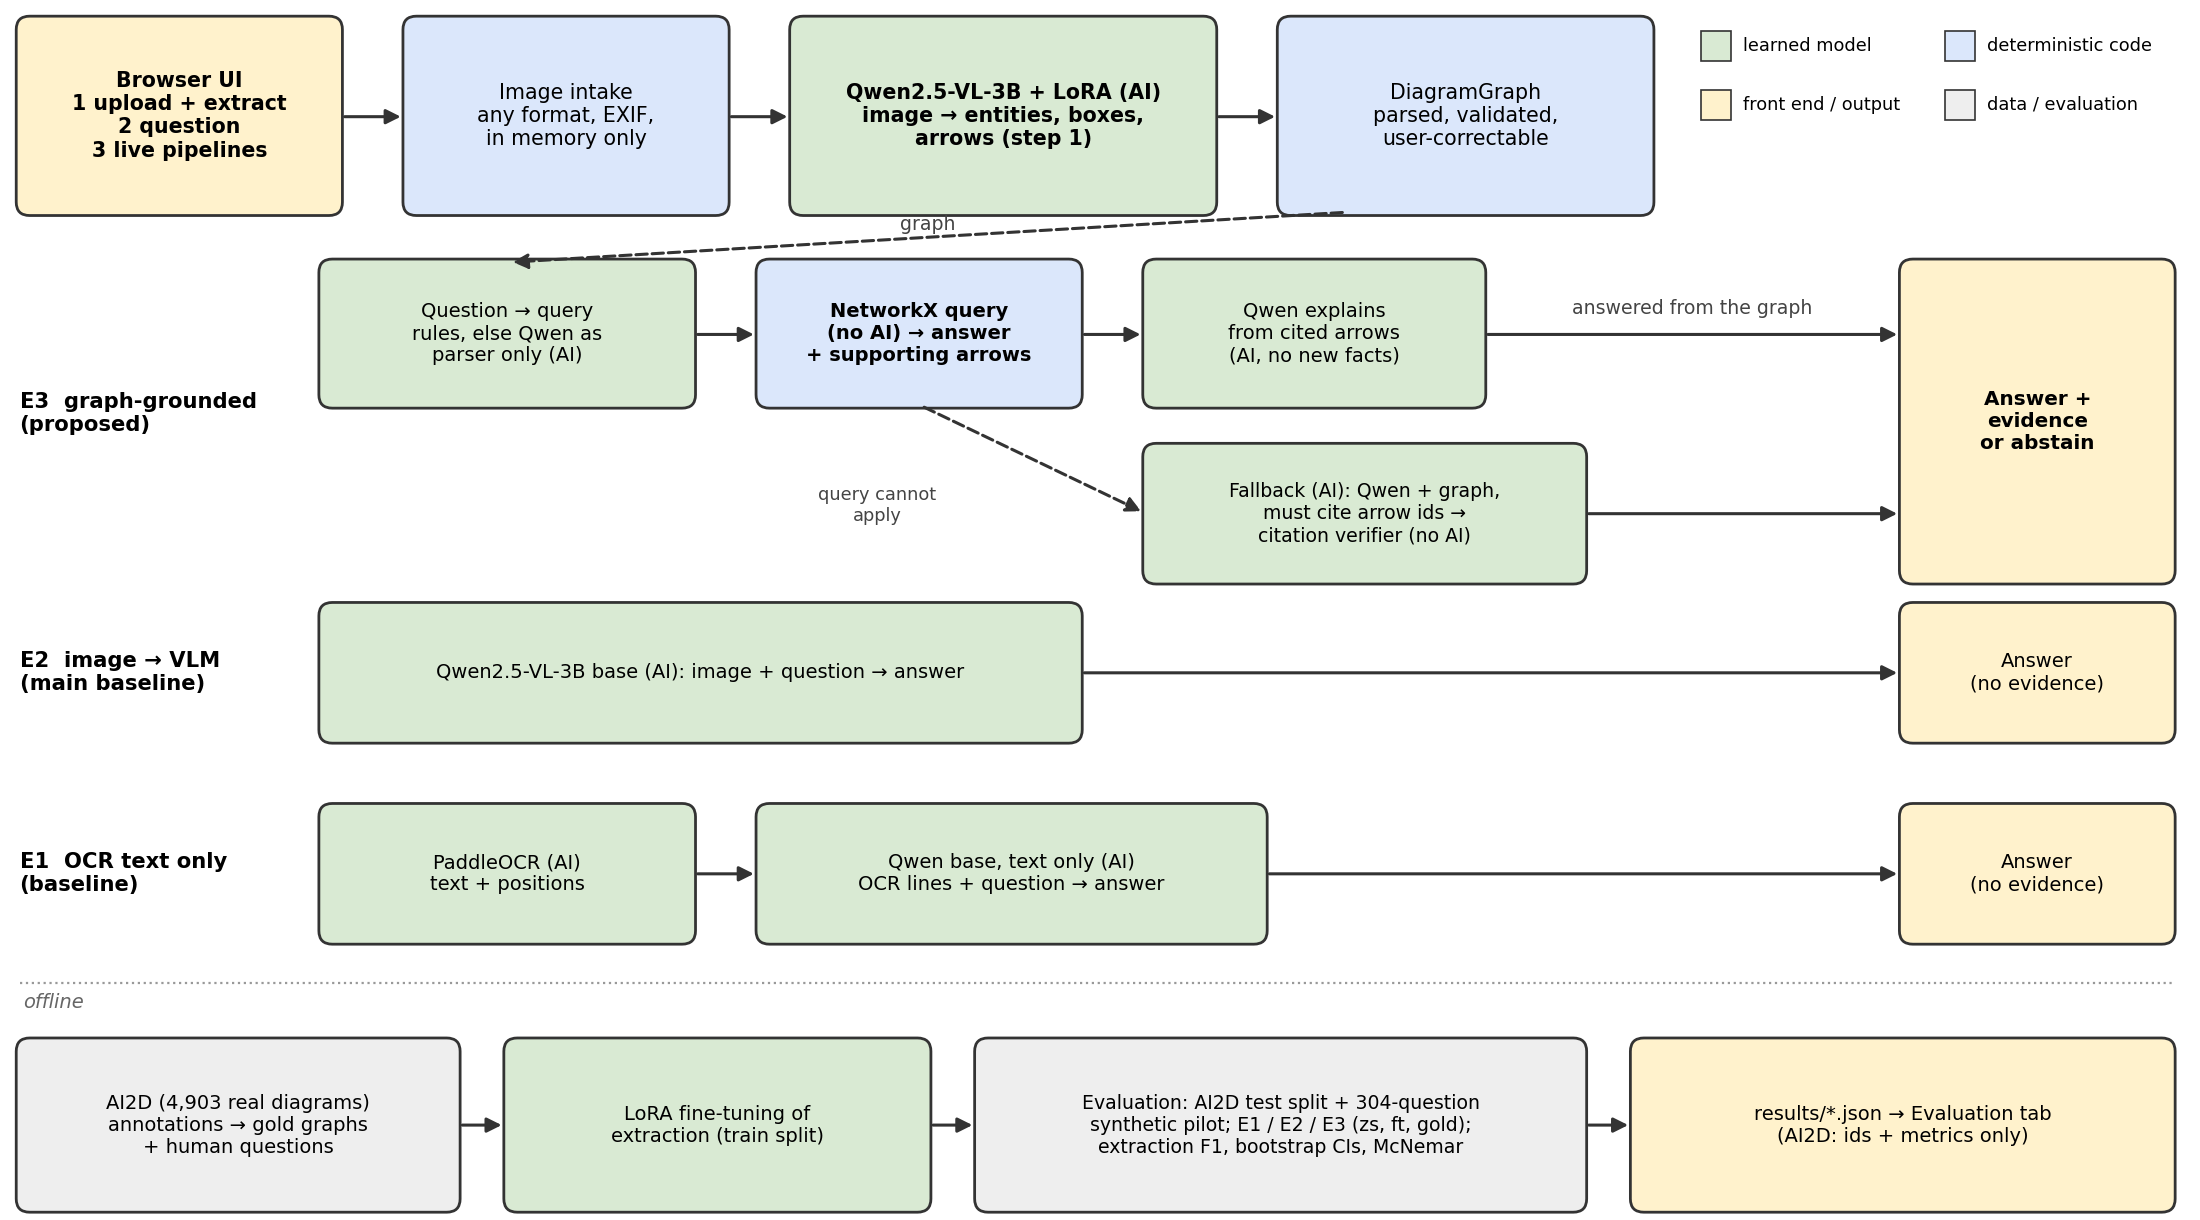
\includegraphics[width=0.93\textwidth]{../../docs/figures/architecture.png}
\end{center}
\vspace{-4pt}
The server is stateless: the graph lives in the browser and is sent back with each question, so student corrections are used immediately.

\section{Data and Model/Algorithm}
\textbf{Data:} 10 synthetic diagrams generated by our seeded script (flowchart, food chain, a \emph{counterfactual} food chain with all arrows reversed, water cycle, web architecture, photosynthesis, and 3 graphs with nonsense labels) with exact gold graphs and 79 templated questions (direct inputs/outputs, arrow checks incl. reversed, paths, and 19 questions whose correct response is to abstain). No third-party data was used in Phase 2; AI2D integration is deferred.
\textbf{Model:} Qwen2.5-VL-3B-Instruct (Qwen Research License: \emph{non-commercial only}; weights not redistributed), one extraction prompt, greedy decoding. \textbf{Algorithm:} deterministic NetworkX queries over the extracted graph. The model does not write E3 answers.

\section{Preliminary Results (pilot, n = 79 questions, 10 diagrams; actual run)}
Method: identical 79 questions for each condition; E2 = Qwen2.5-VL-3B answers from the image; E3 = Qwen extracts the graph, deterministic QA answers; E3* = gold graph + same QA. One run on an Apple M4 (MPS). Raw outputs and scoring rules in \texttt{results/} and \texttt{docs/evaluation.md}.

{\small
\begin{tabularx}{\textwidth}{@{}Lrrrr@{}}
\toprule
\textbf{Question kind (n)} & \textbf{E2 direct VLM} & \textbf{E3 VLM graph + QA} & \textbf{E3* gold graph} \\
\midrule
Direct inputs / outputs (30) & 20 (67\%) & 17 (57\%) & 30 \\
Arrow drawn A$\rightarrow$B: ``Does A point to B?'' (10) & 9 (90\%) & 7 (70\%) & 10 \\
Reversed: ``Does B point to A?'' (10) & \textbf{1 (10\%)} & \textbf{8 (80\%)} & 10 \\
Path exists? (10) & 7 (70\%) & 6 (60\%) & 10 \\
Should abstain (19) & 12 (63\%) & 16 (84\%) & 19 \\
\midrule
\textbf{All (79)} & \textbf{49 (62\%)} & \textbf{54 (68\%)} & \textbf{79 (100\%)} \\
\bottomrule
\end{tabularx}}

\textbf{Extraction:} entity F1 1.00, directed-edge F1 0.68 (P 0.70, R 0.67); 5/10 diagrams perfect; 8 reversed edges, 5 on the counterfactual diagram, where Qwen output the biologically ``expected'' arrows instead of the drawn ones. Mean latency 86\,s per extraction, 16\,s per direct answer.
\textbf{Interpretation:} E3 vs E2 is \emph{not} significant at this size (21 discordant questions, 13 vs 8; exact sign test $p=0.38$). Observed: E2 answers ``Yes'' to 9/10 reversed-arrow questions; E3 cites the opposite arrow. All E3 errors come from extraction (E3* = 100\% on templated questions the rules were built for). \textbf{Demo:} a new JPEG (thermostat loop) was extracted fully correctly; ``What feeds into Sensor?'' abstained; in the UI, deleting the wrong Grass$\rightarrow$Rabbit edge and adding Rabbit$\rightarrow$Grass fixed the answer (Fig.~2).

\begin{center}
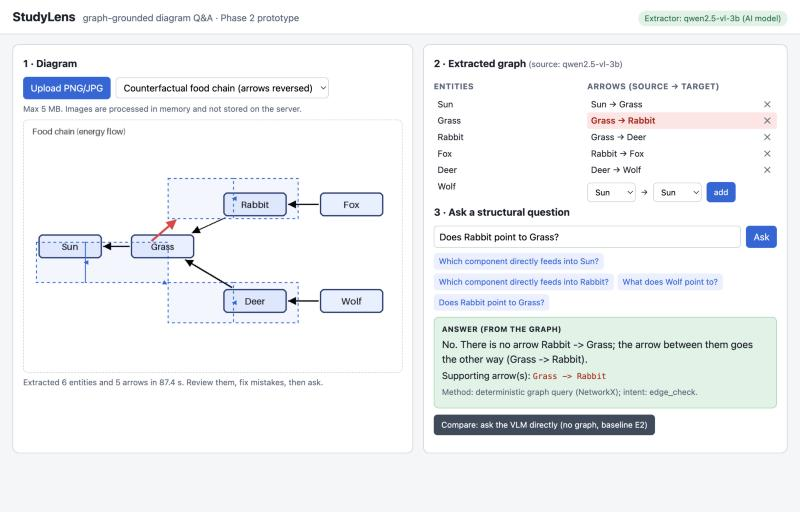
\includegraphics[width=0.49\textwidth]{../../docs/figures/ui_counterfactual_extraction_error.jpg}\hfill
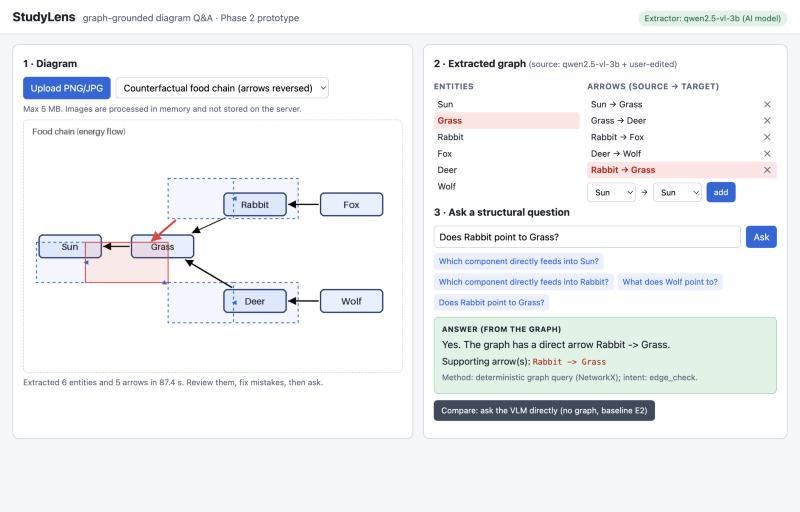
\includegraphics[width=0.49\textwidth]{../../docs/figures/ui_after_user_correction.jpg}\\[-1pt]
{\small\textbf{Figure 2.} Actual prototype screenshots (qwen backend). Left: Qwen extracted Grass$\rightarrow$Rabbit although the drawn arrow points Rabbit$\rightarrow$Grass; the cited evidence edge (red) visibly contradicts the image. Right: after the user corrects the edge, the graph-grounded answer is ``Yes'' with evidence Rabbit$\rightarrow$Grass.}
\end{center}

\section{Known Limitations}
\begin{itemize}
\item Graph QA is only as good as the extracted graph: wrong edges give confident, wrong but \emph{inspectable} answers (20 of 25 E3 errors). Edge direction on unfamiliar or counterfactual diagrams is the main weakness.
\item Rule-based question parser: supports listed structural intents only; not tested on free-form paraphrases. Approximate VLM boxes; no confidence scores; $\sim$1.5\,min per diagram on a laptop.
\item Evaluation is a small synthetic pilot (one run, string-matched E2 scoring checked by hand); no AI2D, OCR (E1) or ablations yet. Qwen2.5-VL-3B is licensed for non-commercial research only.
\end{itemize}

\section{Remaining Tasks (Phase 3)}
\begin{itemize}
\item Scale evaluation: AI2D subset (licence to confirm), Hou et al.\ diagrams, a larger counterfactual set, paraphrased/free-form questions, and paired bootstrap CIs for E2 vs E3.
\item Improve extraction direction accuracy: arrowhead-focused prompting, two-pass extraction, OCR (PaddleOCR) for labels, and ablations (no OCR / no coordinates); optional LoRA (E4).
\item Flag low-confidence or contradictory edges for user review; an LLM fallback for question parsing that still answers only through graph queries.
\item Demo video, failure analysis, final report.
\end{itemize}

\section{Team Responsibilities}
\textbf{Krish Patel} (sole team member, as in Phase 1): all current work, including extraction, graph QA, web app, synthetic data, evaluation, documentation and reports. \todo{Confirm, or add members and their roles.}

\end{document}
